\documentclass[aspectratio=169,10pt]{beamer}
\usepackage{graphicx}
\usepackage{booktabs}
\usepackage{array}
\usepackage{amsmath}
\graphicspath{{../figures/}}

%,- red colour theme (as collab_talk_imperial_2026.tex),-
\definecolor{ubred}{RGB}{160,20,20}
\definecolor{ubdark}{RGB}{90,10,10}
\definecolor{ublight}{RGB}{205,70,70}
\usetheme{default}
\usecolortheme{default}
\setbeamercolor{structure}{fg=ubred}
\setbeamercolor{title}{fg=ubdark}
\setbeamercolor{frametitle}{fg=white,bg=ubred}
\setbeamercolor{section in head/foot}{fg=white,bg=ubdark}
\setbeamercolor{alerted text}{fg=ubred}
\setbeamercolor{block title}{fg=white,bg=ubred}
\setbeamercolor{block body}{bg=ubred!8}
\setbeamercolor{itemize item}{fg=ubred}
\setbeamercolor{itemize subitem}{fg=ublight}
\setbeamertemplate{navigation symbols}{}
\setbeamertemplate{frametitle}{\vskip4pt\usebeamercolor[fg]{frametitle}%
  \begin{beamercolorbox}[wd=\paperwidth,ht=2.4ex,dp=1ex,leftskip=.3cm]{frametitle}%
  \bfseries\insertframetitle\end{beamercolorbox}}
\newif\ifbackup
\setbeamertemplate{footline}{%
  \leavevmode\hbox{%
  \begin{beamercolorbox}[wd=.62\paperwidth,ht=2.4ex,dp=1ex,leftskip=.3cm]{section in head/foot}%
  \usebeamerfont{author in head/foot}\insertshortauthor\ | MicroBooNE NuMI CC$1\mu1\pi^{\pm}$\hfill\end{beamercolorbox}%
  \begin{beamercolorbox}[wd=.38\paperwidth,ht=2.4ex,dp=1ex,rightskip=.3cm]{section in head/foot}%
  \hfill\insertshorttitle\quad\ifbackup Backup \insertframenumber\else\insertframenumber\,/\,\pageref{mainend}\fi\end{beamercolorbox}}}

\title[CC$1\mu1\pi^{\pm}$ update]{Differential CC$\,1\mu1\pi^{\pm}$ cross sections on argon in the NuMI beam}
\subtitle{Updates since the collaboration meeting: releases 1.6 to 1.9}
\author[Pophale, Nowak]{Ishanee Pophale and Jarek Nowak}
\institute{Lancaster University}
\date{October 2026}
\newcommand{\GeVc}{\ensuremath{\,\mathrm{GeV}/c}}

\begin{document}

{\setbeamertemplate{footline}{}
\begin{frame}[plain]
  \titlepage
  \begin{center}\small\color{ubdark}
  $\nu_\mu+\bar\nu_\mu$ CC single charged pion on argon \;$\bullet$\; FHC, RHC and combined \;$\bullet$\; signal region blind,
  results on pseudo-data\\[3pt]
  \footnotesize Previous report: MicroBooNE Collaboration Meeting, Imperial College London, 12--17 September 2026
  \end{center}
\end{frame}}

% ---------------------------------------------------------------------------
\begin{frame}{Since the collaboration meeting}
  \small
  \begin{tabular}{p{0.15\textwidth}p{0.78\textwidth}}
    \toprule
    Date & Change \\
    \midrule
    18--19 Sep & FHC Run-1 beam-on exposure corrected (no open-trigger data): $3.283\to2.192\times10^{20}$~POT; rebuild \\
    09 Sep--1 Oct & Control regions compared with beam-on data under a frozen protocol; corrections to the sideband simulation \\
    26 Sep & Binning review: the $0.50$ migration criterion for both families, $\theta_\mu$ dropped, $p_p$ added \\
    18--28 Sep & New results ($\theta_p$, $\theta_{\pi p}$, two combined-only 2D) and four status labels; validation V1 \\
    29 Sep & Version 1.6: Editorial Board package (three documents) \\
    1 Oct & Version 1.6.1: dirt normalisation in the count and control-region macros \\
    5 Oct & Version 1.7: Bragg-pion cut dropped (missing in the older data productions) \\
    9 Oct & Version 1.8: detector variations applied fractionally (samples simulated with the old NuMI flux) \\
    11--16 Oct & Version 1.9: MCS calibration of exiting muons from the control regions, hold-out test \\
    \bottomrule
  \end{tabular}\\[2mm]
  \footnotesize Versions 1.7 to 1.9 tagged on 14 October. Every result is still extracted from pseudo-data; the signal region is blind.
\end{frame}

\begin{frame}{At the meeting and now}
  \footnotesize\setlength{\tabcolsep}{4pt}
  \begin{tabular}{lp{0.40\textwidth}p{0.40\textwidth}}
    \toprule
    & Collaboration meeting (Draft 1.5) & Version 1.9 \\
    \midrule
    Exposure ($10^{20}$ POT) & FHC $8.857$, RHC $11.082$, comb.\ $19.939$ & FHC $7.766$, RHC $11.082$, comb.\ $18.848$ \\
    Efficiency, purity & $17.4$--$17.6\%$, $57.7$--$58.5\%$ (Bragg-$\pi$ cut) & $18.3$--$18.4\%$, $56.6$--$57.3\%$ (no Bragg-$\pi$ cut) \\
    Binning criterion & diagonal $\geq0.68$ ($p_\mu$ exempt) & $\geq0.50$ for every released observable \\
    Inclusive observables & $p_\mu$ 7, $\cos\theta_\mu$ 5, $\theta_\mu$ 5, $\cos\theta_\pi$ 5, $\theta_{\mu\pi}$ 5, $p_\pi$ 2 &
      $p_\mu$ 5, $\cos\theta_\mu$ 8, $\cos\theta_\pi$ 5, $\theta_{\mu\pi}$ 5, $p_\pi$ 3, 2D $\cos\theta_\pi\times\cos\theta_\mu$ \\
    Inclusive totals & $1.03/0.93/0.97$, $\pm37.6$--$38.7\%$ & $1.042/0.925/0.975$, $\pm34.1$--$35.9\%$ \\
    Proton-tagged totals & $0.62/0.53/0.57$, $\pm40$--$47\%$ & $0.618/0.522/0.563$, $\pm40.5$--$42.9\%$ \\
    Validation & closure $1.010$; 32 throws; no alternative model & closure $1.003$; 100--500 members; two reweighted models \\
    Control regions & pseudo-data only; request to open & beam-on: global $7.69/8$ ($p=0.46$); all shape tests pass \\
    Detector variations & absolute differences & fractional (DVfrac) \\
    MCS momentum & $\pm5\%$ scale term & calibration from the control regions, term \texttt{cov\_MCScal} \\
    \bottomrule
  \end{tabular}\\[1mm]
  {\scriptsize Totals in $10^{-38}$~cm$^2$/Ar (FHC/RHC/combined), on pseudo-data.}
\end{frame}

% ===========================================================================
\section{Exposure and control regions}

\begin{frame}{FHC Run-1 exposure}
  \begin{columns}[T]
  \column{.55\textwidth}
  \begin{itemize}\footnotesize\setlength\itemsep{3pt}
    \item In the control regions FHC Run~1 sat at data/prediction $0.60$--$0.72$; a free exposure factor fitted
          $0.520\pm0.020$.
    \item Cause: our Run-1 beam-on file holds no open-trigger data; its exposure is $2.192\times10^{20}$~POT and
          $5\,748\,692$ triggers, not $3.283\times10^{20}$ and $9\,846\,635$ (the open-trigger share, runs 3490--4950).
          Confirmed against the beam bookkeeping and the file transfer.
    \item Adopted: FHC $8.857\to7.766\times10^{20}$, combined $19.939\to18.848\times10^{20}$~POT; combined flux
          $6.60865\to6.59691\times10^{-10}$; FHC beam-off $30.2\to23.2$ events; about 20 hard-coded scales fixed.
    \item 34 universe files rebuilt. On pseudo-data the integrals move by $0.95$--$1.05$ (the exposure cancels); on
          beam-on data the correction raises $\sigma_{\rm FHC}$ by $14.0\%$ and $\sigma_{\rm comb}$ by $5.8\%$.
    \item Control-region global $\chi^2$: $69.5/8\to8.1/8$.
    \item Still open: a free Run-1 factor fits $0.869\pm0.022$ ($\Delta\chi^2=37$); cause not identified.
  \end{itemize}
  \column{.43\textwidth}
  \centering\includegraphics[width=\textwidth]{bkgfit/data_fR1_profile}\\
  {\scriptsize $\Delta\chi^2$ profile of the FHC Run-1 exposure factor in the control regions.}
  \end{columns}
\end{frame}

\begin{frame}{Control regions with beam-on data: frozen protocol}
  \begin{columns}[T]
  \column{.52\textwidth}
  \begin{itemize}\footnotesize\setlength\itemsep{2pt}
    \item Four inclusive control regions (CC$0\pi$, $\pi^0$, multi-$\pi$, cosmic), FHC Runs 1, 4, 5 and RHC Runs 1, 3, 4
          (no Run-2 beam-on file); signal region excluded from the skim.
    \item Frozen protocol: global normalisation $\chi^2$ (8 regions), pulls, shape tests in $p_\mu$, $\cos\theta_\mu$
          and a third variable per region.
    \item Corrections before interpreting: the sideband simulation predated the beam-frame fix (FHC CC$0\pi$
          $\cos\theta_\mu$ $350.5/4\to3.26/4$, an artefact); the sideband detector variations were not POT-normalised
          (detector term $\approx20\%\to1$--$2\%$).
  \end{itemize}
  \vspace{1mm}
  \scriptsize\setlength{\tabcolsep}{3pt}
  \begin{tabular}{lc}
    \toprule
    Global normalisation $\chi^2$ (beam-on) & \\
    \midrule
    first comparison (9 Sep) & $8.77/8$ \\
    corrected detector term, old Run-1 exposure & $69.5/8$ \\
    corrected Run-1 exposure & $8.11/8$ \\
    dirt fix (v1.6.1) & $6.03/8$ \\
    v1.7 selection, unchanged in v1.9 & $7.69/8$ ($p=0.46$) \\
    \bottomrule
  \end{tabular}
  \column{.46\textwidth}
  \centering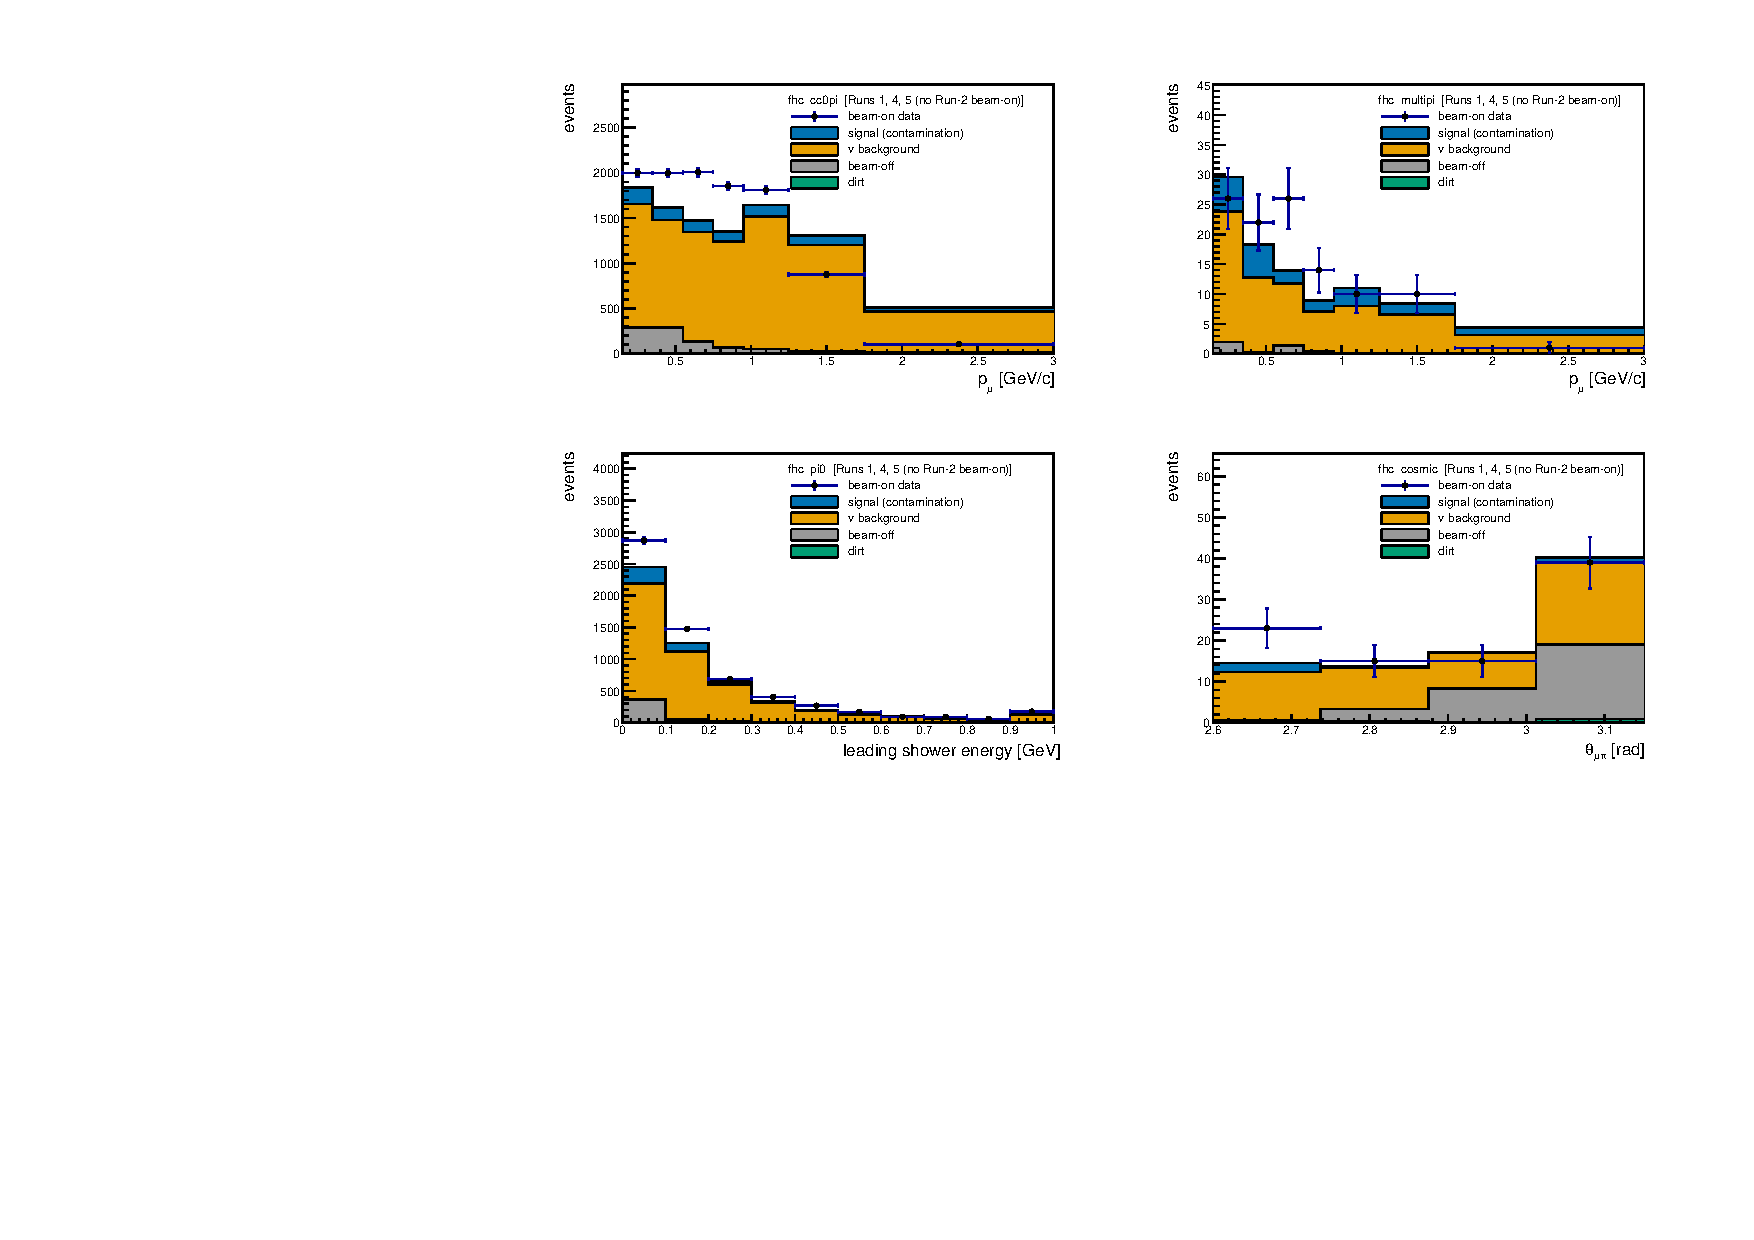
\includegraphics[width=\textwidth]{sideband_data_fhc_compact}\\
  {\scriptsize FHC control regions, beam-on data against the prediction (v1.7 simulation, before the MCS calibration).}
  \end{columns}
\end{frame}

\begin{frame}{Control regions: background fit, constraint, far sidebands}
  \begin{columns}[T]
  \column{.50\textwidth}
  \begin{itemize}\footnotesize\setlength\itemsep{3pt}
    \item Joint FHC+RHC background fit: CC$0\pi$ scale $0.991\pm0.190$ (v1.7); no correction warranted, FHC and RHC
          agree. The other periods sit $8$--$23\%$ above prediction in CC$0\pi$ and $\pi^0$, inside the flux and
          cross-section terms.
    \item Conditional constraint of the one-bin total from the control regions (Asimov): $35.8\%\to11.3\%$, entirely
          through the flux and detector correlations. Adopting it needs a collaboration decision.
    \item Far sidebands (one extra cut per region): CC$0\pi$ signal fraction $8.6\%\to2.2\%$ keeping $58\%$ of the
          events; data/prediction CC$0\pi$ $1.09$--$1.13$, far cosmic $0.76$ (the data prefer less dirt).
    \item The residuals are organised in $p_\mu$: the symptom of the MCS mis-modelling (next section).
  \end{itemize}
  \column{.48\textwidth}
  \centering\includegraphics[width=\textwidth]{bkgfit/data_residuals}\\
  {\scriptsize Data over prediction in $\cos\theta_\mu\times p_\mu$ groups after the fit.}
  \end{columns}
\end{frame}

% ===========================================================================
\section{Binning and new results}

\begin{frame}{Binning review: the 0.50 criterion}
  \begin{columns}[T]
  \column{.52\textwidth}
  \begin{itemize}\footnotesize\setlength\itemsep{2pt}
    \item 141 candidate binnings extracted in FHC, RHC and combined; maximin partition by dynamic programming, scored
          by the trace of $A_C$ (degrees of freedom of the signal); the fewest bins reaching $90\%$ of the largest
          admissible trace.
    \item The released $p_\mu$ (diagonal $0.33$) and $W_{\rm had}$ ($0.09$) failed both criteria; $\cos\theta_\mu$ and
          $\theta_\mu$ failed $0.68$.
    \item Adopted 26 September: $0.50$ for both families.
  \end{itemize}
  \vspace{1mm}
  \scriptsize\setlength{\tabcolsep}{3pt}
  \begin{tabular}{lll}
    \toprule
    Observable & Meeting & Now \\
    \midrule
    $p_\mu$ & 7 bins & 5 (6, then the MCS merge) \\
    $\cos\theta_\mu$ & 5 & 8 \\
    $p_\pi$ & 2 & 3 regions ($0.175, 0.205, 0.26$, open) \\
    $\theta_\mu$ & 5 & dropped \\
    $W_{\rm had}$ & 6 & 2 (split $1.18$) \\
    $\delta\phi_T$ & 2 & 3 \\
    $\theta_p$, $\theta_{\pi p}$ & n/a, 3 & 4, 4 \\
    $p_p$ & n/a & 3 ($0.3, 0.42, 0.60$, open) \\
    \bottomrule
  \end{tabular}
  \column{.46\textwidth}
  \centering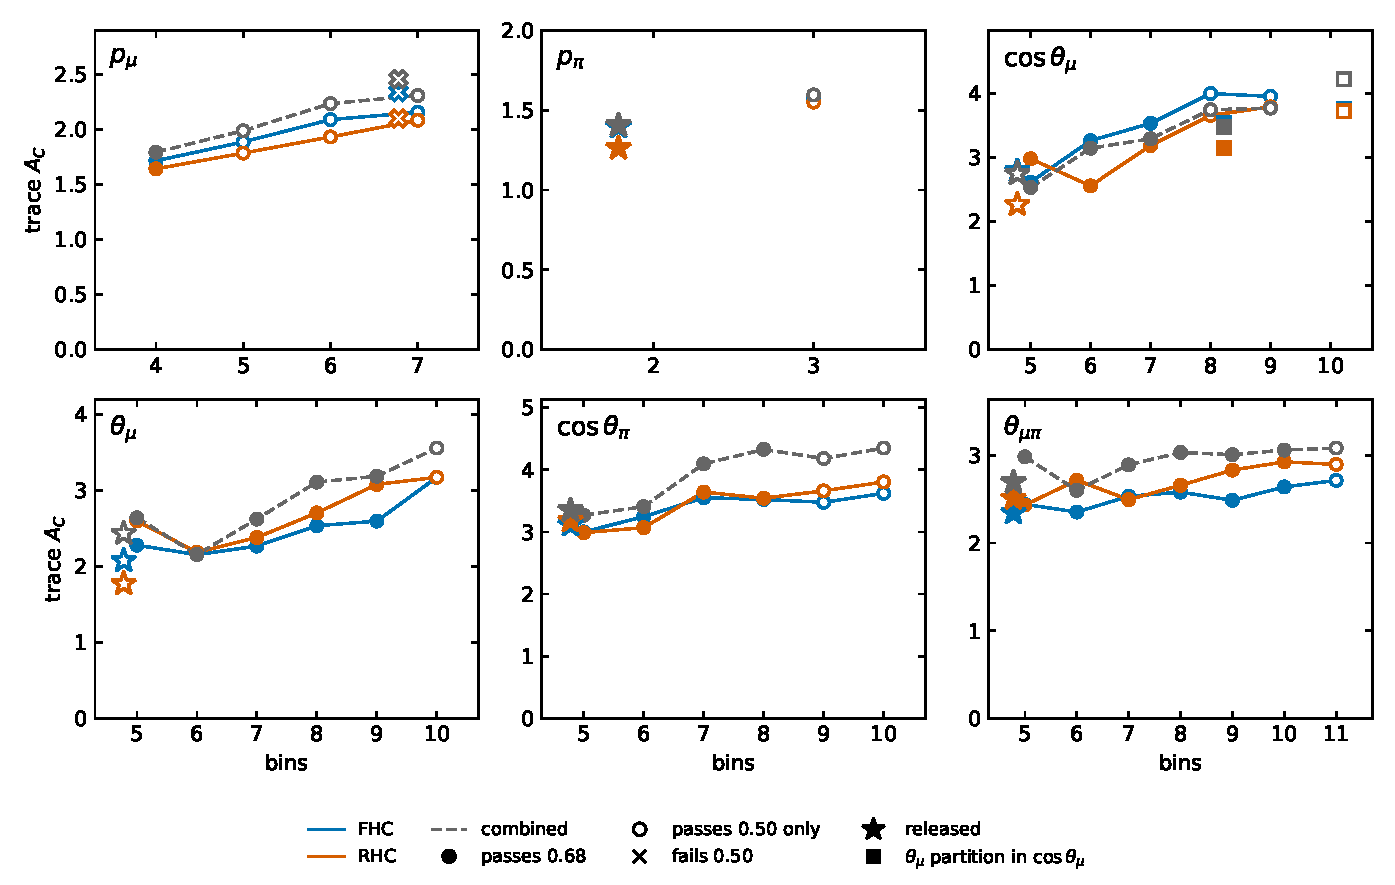
\includegraphics[width=\textwidth]{binreview_dfs_incl}\\
  {\scriptsize $A_C$ degrees of freedom against the number of bins, inclusive observables.}
  \end{columns}
\end{frame}

\begin{frame}{New results and status labels}
  \begin{columns}[T]
  \column{.44\textwidth}
  \begin{itemize}\footnotesize\setlength\itemsep{3pt}
    \item New: $\theta_p$ and $\theta_{\pi p}$ (proton-tagged), and two 2D results in the combined configuration
          only, $\cos\theta_\pi\times\cos\theta_\mu$ (6 cells) and $\theta_p\times\delta p_T$ (4 cells).
    \item The proton candidate is the leading proton in $81.7\%$ of events; wrong picks supply $74\%$ of the
          $\theta_p$ migration.
    \item Four status labels, one source (\texttt{status.tsv}):
    \begin{itemize}\footnotesize
      \item primary: inclusive differentials and total;
      \item secondary: proton-tagged total, $\theta_p$, $\theta_{\pi p}$, both 2D;
      \item validation only: $W_{\rm had}$, TKI, $p_p$, proton-tagged $\mu$/$\pi$ kinematics;
      \item not reported: $\theta_\mu$, 5-bin $p_\pi$, $W_{\pi p}$.
    \end{itemize}
    \item Validation V1 of the new results: widths $0.94$--$1.04$, bias $\leq0.79\sigma$. The release has 59 extractions.
  \end{itemize}
  \column{.54\textwidth}
  \centering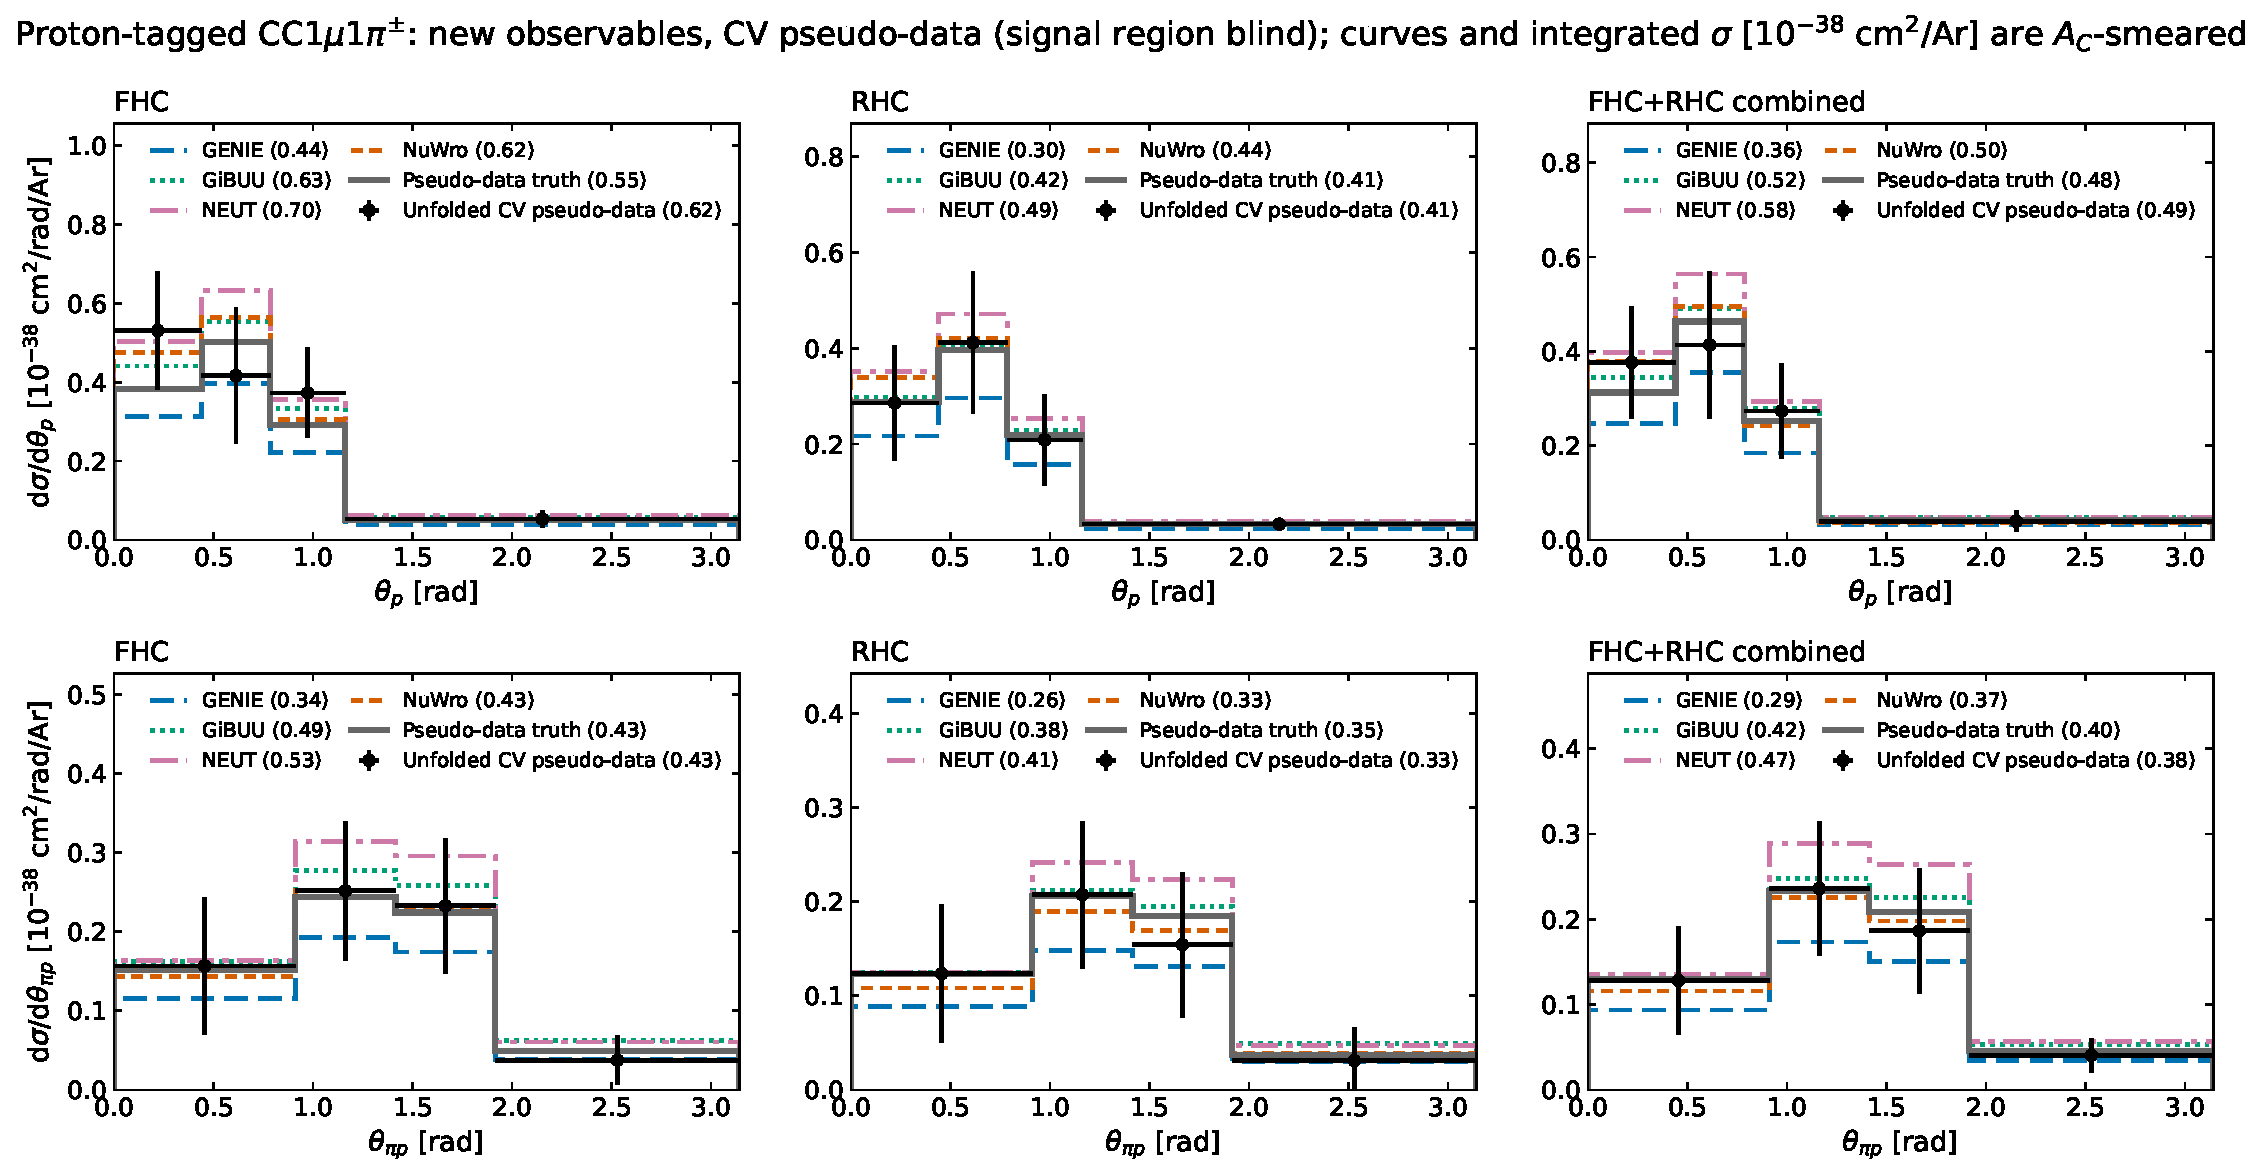
\includegraphics[width=\textwidth]{newobs_xsec}\\
  {\scriptsize $\theta_p$ and $\theta_{\pi p}$ on pseudo-data with the tune and four generators.}
  \end{columns}
\end{frame}

% ===========================================================================
\section{Releases 1.6.1 to 1.8}

\begin{frame}{Dirt normalisation (1.6.1) and the Bragg-pion cut (1.7)}
  \begin{columns}[T]
  \column{.48\textwidth}
  \textbf{\color{ubred}Dirt in the count macros (1 Oct)}
  \begin{itemize}\footnotesize\setlength\itemsep{2pt}
    \item The count and control-region macros scaled the Run-1 dirt by data POT over overlay POT and applied the
          $0.65$ weight twice: dirt $6$--$21\times$ too small. The extraction was never affected.
    \item Signal-region dirt $1.1/1.0/2.1\to6.6/9.5/16.0$ events; purity $-0.3$ points. CR dirt, FHC CC$0\pi$:
          $49\to342$.
    \item CR $\chi^2$: pseudo-data $0.66\to2.29/8$, beam-on $8.11\to6.03/8$. A $100\%$ dirt variation moves the
          totals by $\leq0.9\%$; no dirt term carried.
  \end{itemize}
  \column{.50\textwidth}
  \textbf{\color{ubred}Bragg-pion cut dropped (5 Oct)}
  \begin{itemize}\footnotesize\setlength\itemsep{2pt}
    \item The older data productions (FHC Run~1, RHC Runs 1 and 3b) lack the Bragg-pion score: the cut was
          fail-open in data and applied in the simulation. The control regions showed $7$--$11\%$ excess there;
          at unblinding the totals would have been $4.7\%$ (inclusive) and $4.6\%$ (proton-tagged) high.
    \item Cut dropped in every sample; full reprocess; 65 universe files rebuilt.
    \item Efficiency $17.5\to18.3$--$18.4\%$, purity $57.3/56.6/56.9\%$; proton-tagged efficiency $11.5\to12.1\%$.
    \item Totals $1.034/0.932/0.975\to1.042/0.925/0.975$; closure $0.996\to1.003$; CR global $7.69/8$.
  \end{itemize}
  \end{columns}
\end{frame}

\begin{frame}{Detector variations and the old NuMI flux (1.8)}
  \begin{columns}[T]
  \column{.50\textwidth}
  \begin{itemize}\footnotesize\setlength\itemsep{3pt}
    \item The Run-4 detector-variation samples were simulated with the earlier NuMI flux: per POT their central value
          predicts $1.27$ (FHC) and $1.51$ (RHC) times the nominal rate, rising to $1.8$--$3$ above $5$~GeV;
          reweighted to the current flux, $0.94$, flat.
    \item The absolute difference between a variation and its central value carried that ratio into the
          covariance. Now each variation's fractional change is applied to the nominal prediction (DVfrac).
    \item Detector term per bin $\times0.70$--$0.78$; totals: detector $19.2$--$22.1\%\to14.0$--$14.3\%$, total
          $37.7$--$38.2\%\to34.1$--$35.9\%$ (inclusive). Central values unchanged.
    \item Integrals $\times1.026$ (median); combined $\cos\theta_\mu$ $A_C$ trace $3.81\to4.23$; D'Agostini/WSVD
          $1.30$--$1.36\to1.27$--$1.30$.
  \end{itemize}
  \column{.48\textwidth}
  \centering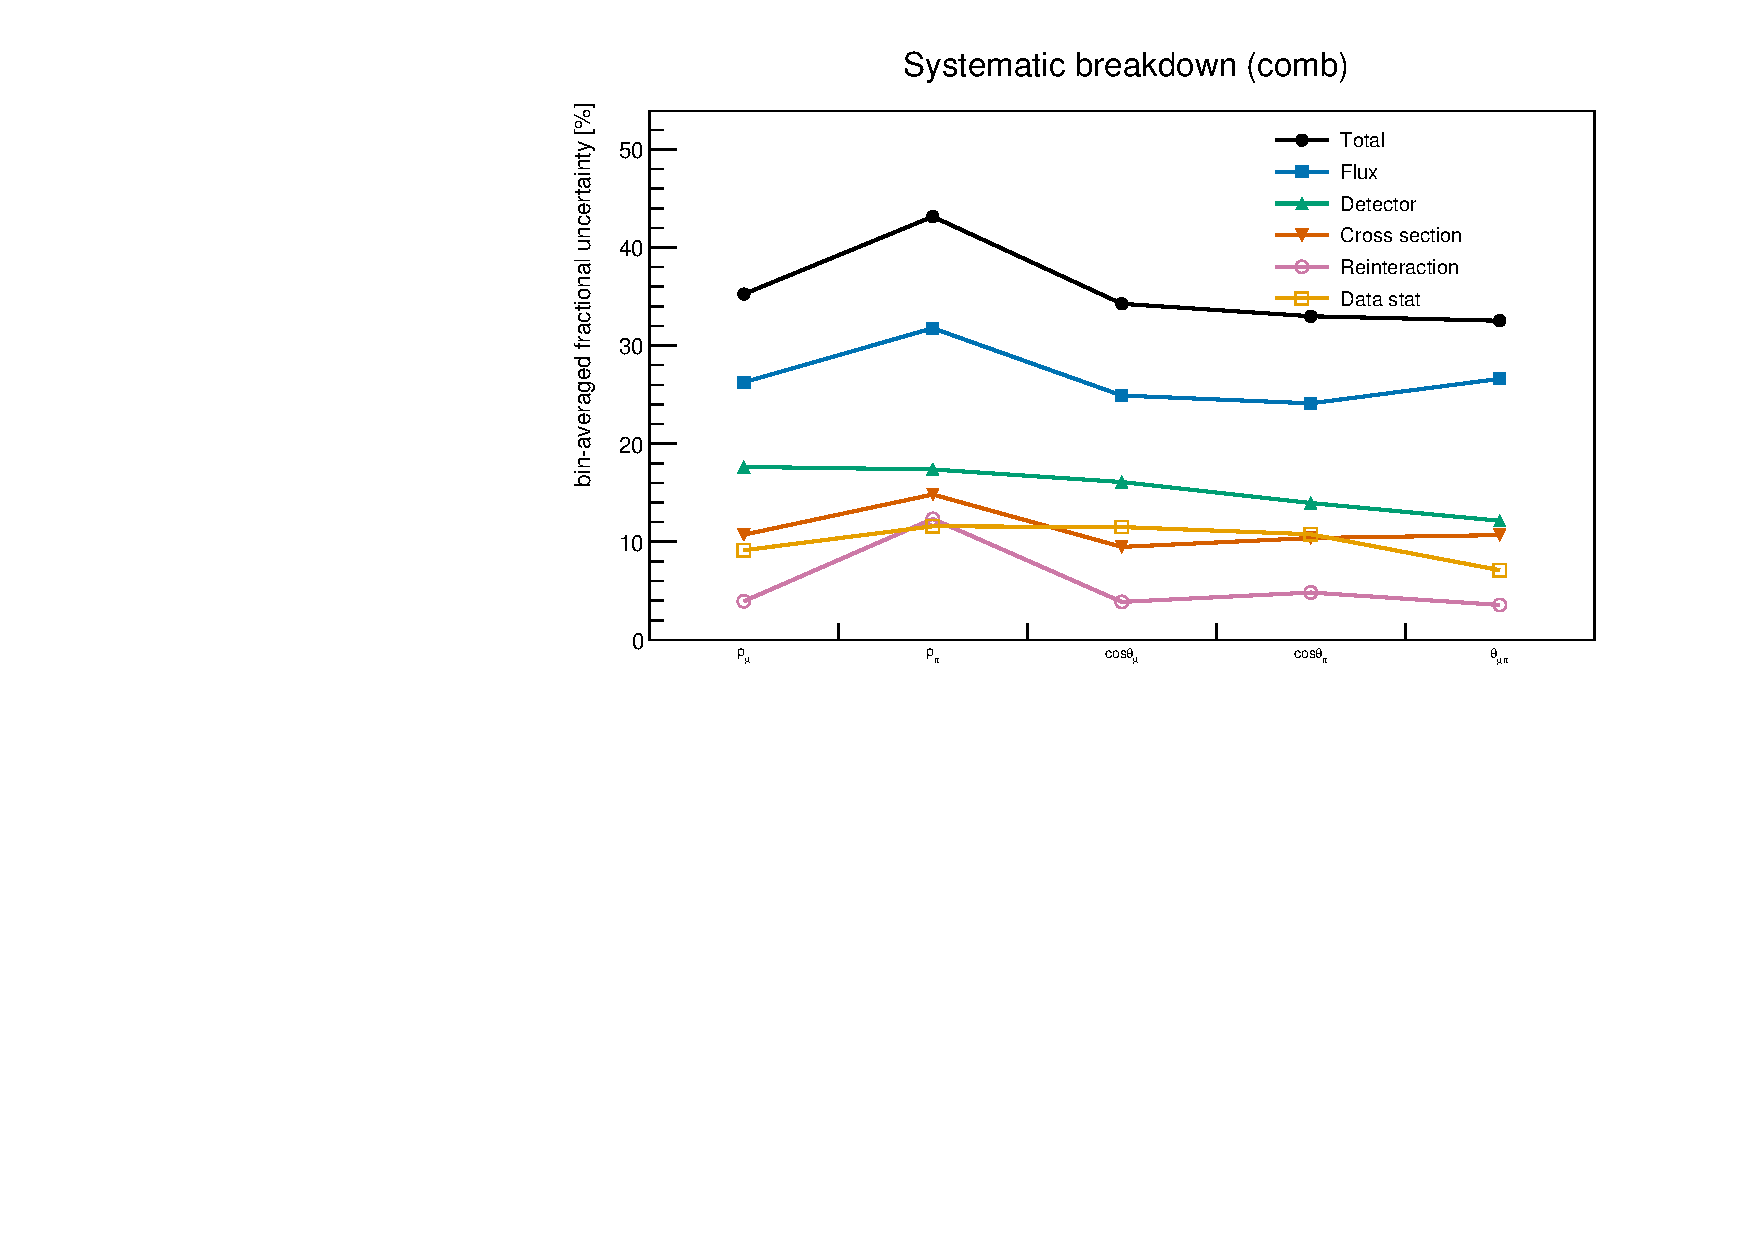
\includegraphics[width=\textwidth]{fw_systbreak_comb}\\
  {\scriptsize Uncertainty breakdown per observable, combined configuration (v1.9).}
  \end{columns}
\end{frame}

% ===========================================================================
\section{MCS calibration}

\begin{frame}{MCS momentum of exiting muons (control regions)}
  \begin{columns}[T]
  \column{.55\textwidth}
  \begin{itemize}\footnotesize\setlength\itemsep{3pt}
    \item Above $1.2\GeVc$ the data hold half the predicted share of exiting muon candidates ($0.157$ against
          $0.318$); data/prediction in the $p_\mu$ bins $1.00$, $1.07$, $1.21$, $1.25$, $1.09$, $0.48$.
    \item Stopping muons agree: MCS over range within $1.5\%$ up to $3\GeVc$, so the momentum scale is fine; the
          exiting tracks are not.
    \item Cause: an angular noise of the reconstructed tracks on the scale of the MCS segments ($5$--$11$~mrad
          equivalent), absent in the simulation, depending on the drift-direction component and the length of the
          track. Only the SCE variation moves the MCS momentum, by about a fifth of the effect.
    \item Uncorrected impact: up to $2.7\sigma$ in a $p_\mu$ bin and $+25$--$29\%$ on the $p_\mu$ integral, against at
          most $0.65\sigma$ from the $\pm5\%$ term then carried.
  \end{itemize}
  \column{.43\textwidth}
  \begin{block}{\small History of the MCS term}\footnotesize
    \begin{itemize}\setlength\itemsep{1pt}
      \item $\pm5\%$/$\pm10\%$ common scale: withdrawn on 19 Sep (it cancels).
      \item Data-side $\pm5\%$ term: $0.34\sigma\to0.65\sigma$ through v1.8; in the official covariance from 27 Sep.
      \item v1.9: calibration from the control regions, term \texttt{cov\_MCScal}.
    \end{itemize}
  \end{block}
  \end{columns}
\end{frame}

\begin{frame}{MCS calibration (1.9)}
  \begin{columns}[T]
  \column{.47\textwidth}
  \begin{itemize}\footnotesize\setlength\itemsep{2pt}
    \item Quantile maps of the MCS momentum in 12 cells ($|\hat d_x|\times$ length), applied to every simulated exiting
          track in every sample; 19 results rebuilt, the other 40 bit-identical.
    \item Uncertainty: seven alternative maps in four fully correlated terms (\texttt{cov\_MCScal}), replacing the
          $\pm5\%$ term; FHC $p_\mu$ term $6.5\%$ (bin average), $\leq0.28\sigma$ (FHC), $0.21\sigma$ (RHC), $0.43\sigma$
          (combined).
    \item $p_\mu$: top two bins merged (5 bins, last $>0.825\GeVc$); $\theta_p\times\delta p_T$ edge $0.8\to0.85$.
    \item Control regions: MCS $\chi^2$ $7937/24\to27/24$; $p_\mu$ data/prediction $1.00$, $1.02$, $1.04$, $1.01$, $0.98$,
          $0.97$; every shape test passes (a closure: the maps come from these events).
    \item Inclusive $p_\mu$ integrals against v1.8: $\times1.110/1.018/1.071$.
  \end{itemize}
  \column{.51\textwidth}
  \centering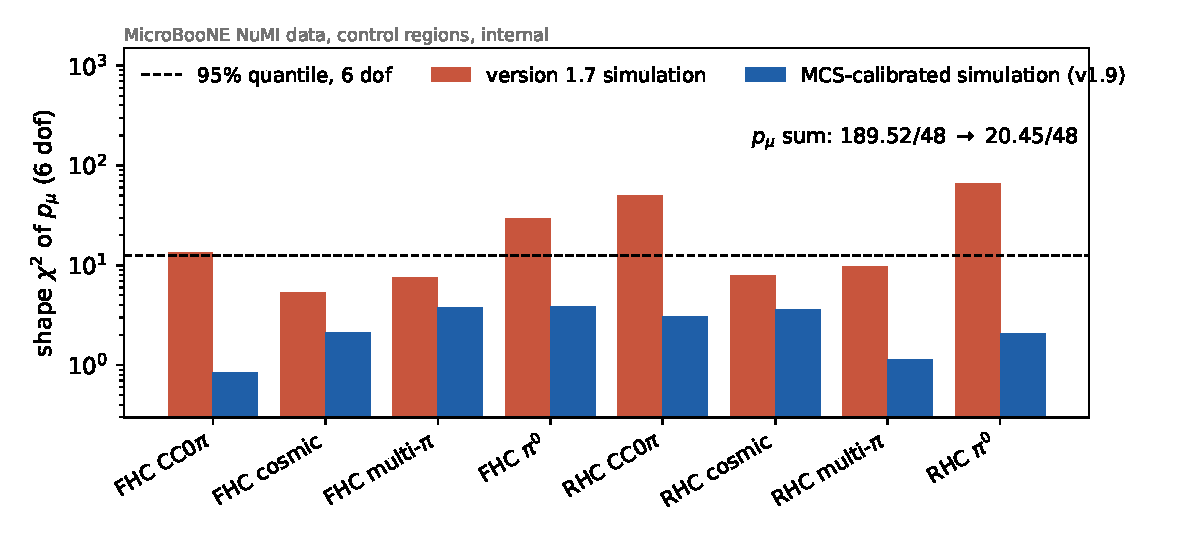
\includegraphics[width=\textwidth]{update_talk/cr_mcscal_chi2}\\
  {\scriptsize Shape $\chi^2$ of $p_\mu$ in the eight control regions, beam-on data, frozen protocol, before and after
  the calibration.}
  \end{columns}
\end{frame}

\begin{frame}{Hold-out test of the calibration}
  \begin{itemize}\small\setlength\itemsep{4pt}
    \item Maps derived from one random half of the control-region events and tested on the other half, and vice
          versa: $p_\mu$ shape $\chi^2$ $21.1/5$ and $5.9/5$, against $7.5\pm4.0$ expected from the statistics of the
          halves alone; the calibrated shares agree within $6\%$.
    \item Transfers between horn modes (FHC to RHC and back) and between productions (older to newer data and back)
          move the top $p_\mu$ bin by $3$--$7\%$, the spread of the period-group maps that build the uncertainty.
    \item The calibration therefore transfers between independent events, horn modes and productions within its
          quoted uncertainty; the closure of the previous slide is not the only evidence.
    \item Record: \texttt{report/results/mcs\_cal\_holdout.\{md,json\}}, \texttt{scripts/mcs\_cal\_holdout.py}.
  \end{itemize}
\end{frame}

% ===========================================================================
\section{Validation and results}

\begin{frame}{Validation}
  \begin{columns}[T]
  \column{.50\textwidth}
  \textbf{\color{ubred}Closure and ensembles}
  \begin{itemize}\footnotesize\setlength\itemsep{2pt}
    \item Closure: inclusive $\chi^2\leq3.12/8$, ratios $0.905$--$1.106$, mean $1.003$ (meeting: $1.010$);
          proton-tagged $\chi^2\leq7.28/4$.
    \item Ensembles: 32 throws at the meeting, then six 100-member ensembles (20 Sep), 500 members for the binning
          review, all rebuilt for v1.7 to v1.9. Widths $0.92$--$1.04$ (inclusive), $0.89$--$1.04$ (proton-tagged);
          offsets within $1.4\%$ at $\leq1.5\sigma$.
    \item 24 Sep: concurrent arrays re-threw shared files and ten members read truncated pseudo-data (RHC total width
          $1.28\to0.99$ after the fix); throws are now created once (\texttt{link(2)}).
  \end{itemize}
  \column{.48\textwidth}
  \textbf{\color{ubred}Alternative models}
  \begin{itemize}\footnotesize\setlength\itemsep{2pt}
    \item Pseudo-data from GENIE multisim universe 545 and the $\Delta\to N\pi$ angular unisim, extracted with the
          nominal response: largest inclusive bias $1.21\sigma$ (FHC $\cos\theta_\mu$ bin 3), RHC $\leq0.90\sigma$;
          proton-tagged low $\delta p_T$/$p_n$ $-1.19/-1.02\sigma$, lower $W_{\rm had}$ $+1.04\sigma$.
    \item Since v1.7 the truth changes come from the universe ratios, not from two separate throws.
    \item NuWro closure dropped (19 Sep): the Run-1 FHC NuWro overlay has a signal rate $1.76\times$ GENIE against
          $1.6$ expected and its production could not be traced. Independent-generator closure (U3) still pending.
  \end{itemize}
  \end{columns}
\end{frame}

\begin{frame}{One-bin totals (1.9)}
  \begin{columns}[T]
  \column{.46\textwidth}
  \scriptsize\setlength{\tabcolsep}{3pt}
  \begin{tabular}{lcc}
    \toprule
    $10^{-38}$~cm$^2$/Ar & Inclusive & Proton-tagged \\
    \midrule
    FHC & $1.042\pm0.374$ ($35.9\%$) & $0.618\pm0.251$ ($40.6\%$) \\
    RHC & $0.925\pm0.316$ ($34.1\%$) & $0.522\pm0.224$ ($42.9\%$) \\
    Combined & $0.975\pm0.337$ ($34.6\%$) & $0.563\pm0.228$ ($40.5\%$) \\
    \bottomrule
  \end{tabular}
  \begin{itemize}\footnotesize\setlength\itemsep{2pt}
    \item FHC inclusive: flux $30.4\%$, detector $14.2\%$, cross section $10.6\%$, reinteraction $3.8\%$, POT $3.4\%$,
          targets $1.7\%$, data statistics $4.4\%$.
    \item Selected / background: $1522/651$, $1881/817$, $3404/1467$; proton-tagged $677/328$, $834/420$, $1510/749$.
    \item FHC generators: GENIE $0.82$, GiBUU $1.13$, NEUT $1.32$, NuWro $1.25$.
    \item Against the meeting: central values within $1\%$; uncertainty $\approx38\%\to34$--$36\%$ (DVfrac). On beam-on
          data the Run-1 correction adds $+14\%$ to FHC.
  \end{itemize}
  \column{.52\textwidth}
  \centering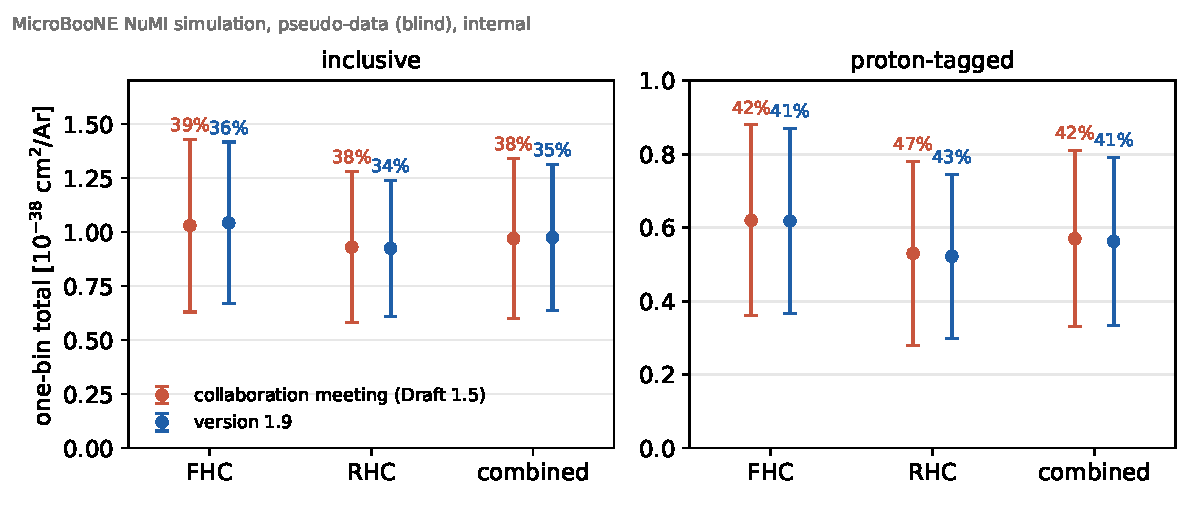
\includegraphics[width=\textwidth]{update_talk/totals_update}
  \end{columns}
\end{frame}

\begin{frame}{Inclusive differential results (1.9)}
  \begin{columns}[T]
  \column{.60\textwidth}
  \centering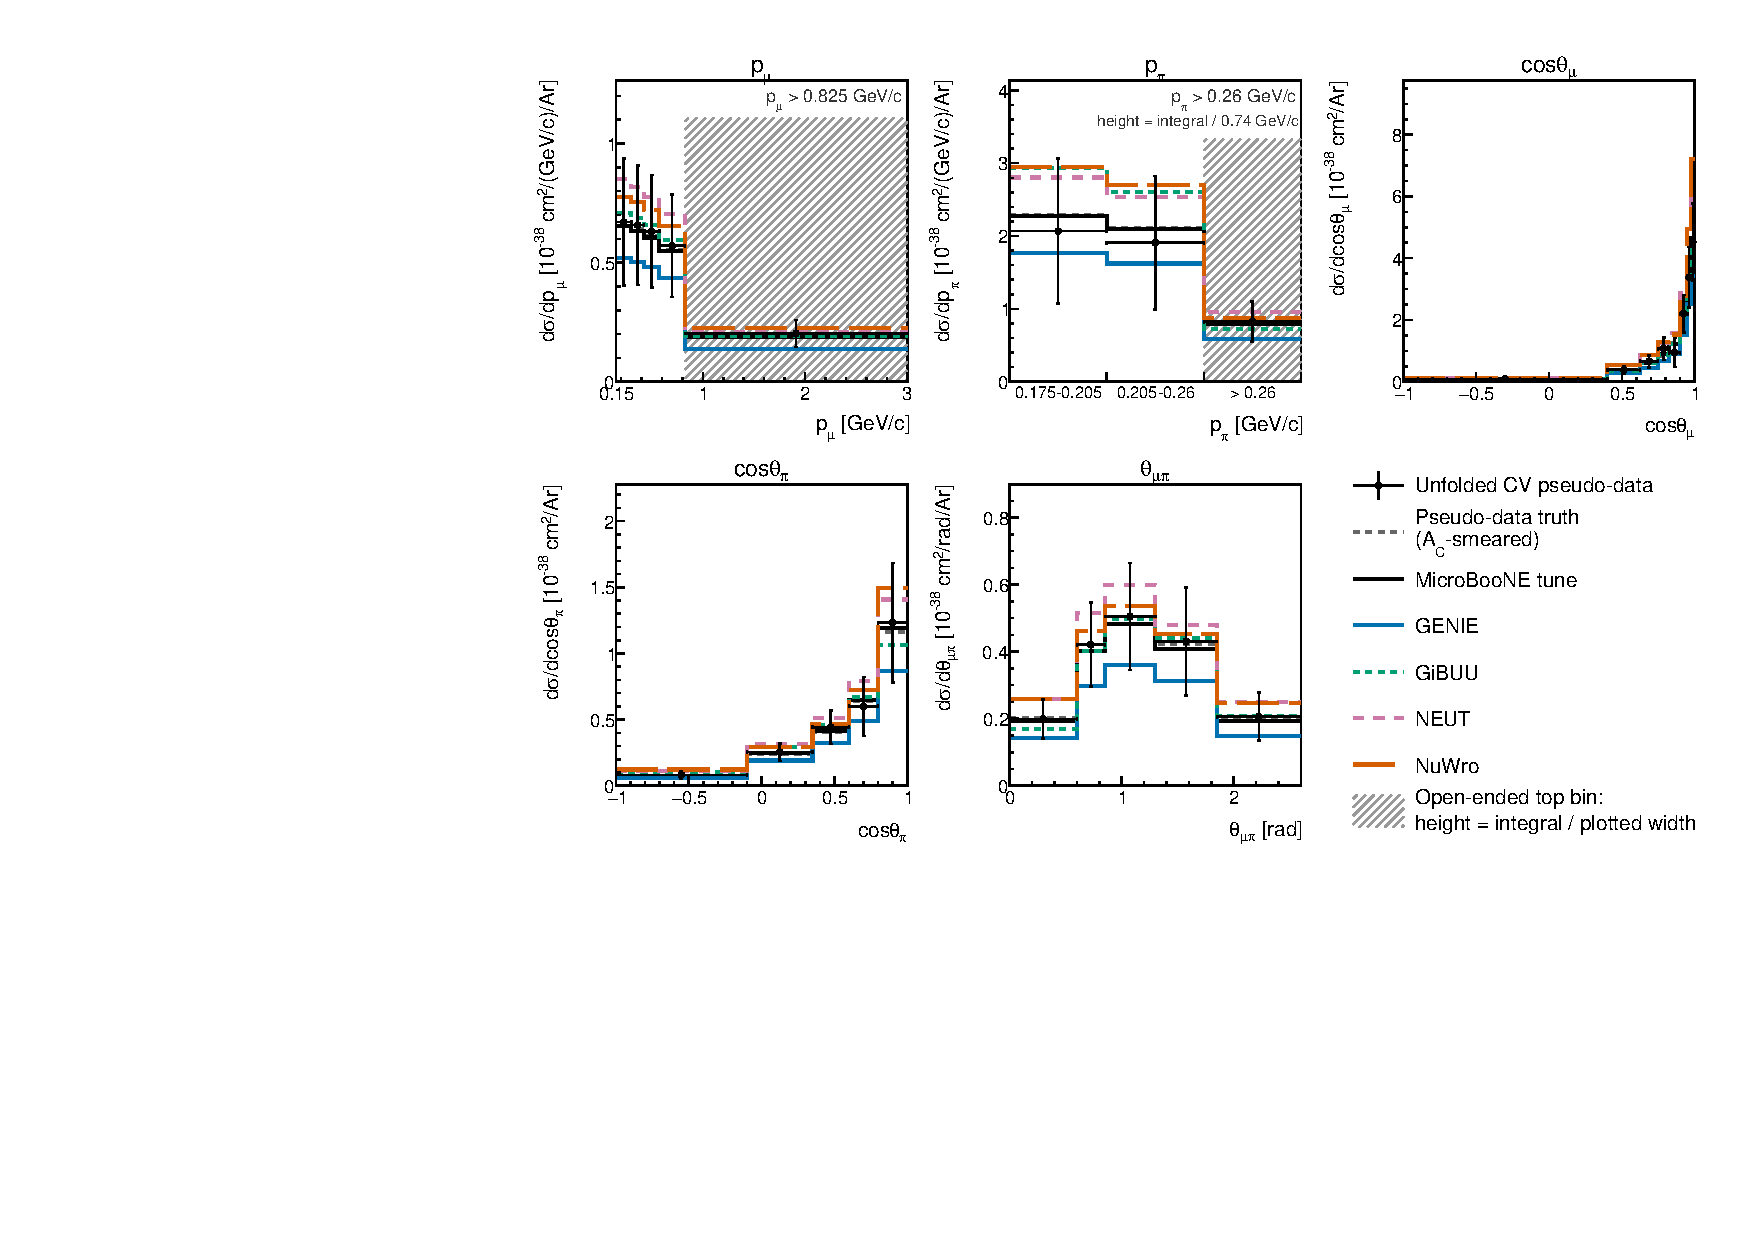
\includegraphics[width=\textwidth]{dsigma_COMB}
  \column{.38\textwidth}
  \begin{itemize}\footnotesize\setlength\itemsep{3pt}
    \item Combined configuration, unfolded pseudo-data with the $A_C$-smeared truth, the tune and four generators.
    \item $p_\mu$ 5, $\cos\theta_\mu$ 8, $\cos\theta_\pi$ 5, $\theta_{\mu\pi}$ 5 bins, $p_\pi$ 3 regions.
    \item Integrals (FHC/RHC/comb.): $p_\mu$ $0.97/0.70/0.86$, $p_\pi$ $0.84/0.74/0.78$, $\cos\theta_\mu$
          $0.72/0.71/0.75$, $\cos\theta_\pi$ $0.66/0.62/0.67$, $\theta_{\mu\pi}$ $0.89/0.81/0.84$ (meeting
          $0.62$--$0.96$).
    \item Bin-averaged systematic total $31$--$49\%$ (meeting: $32$--$54\%$ total).
  \end{itemize}
  \end{columns}
\end{frame}

\begin{frame}{Proton-tagged results (1.9)}
  \begin{columns}[T]
  \column{.60\textwidth}
  \centering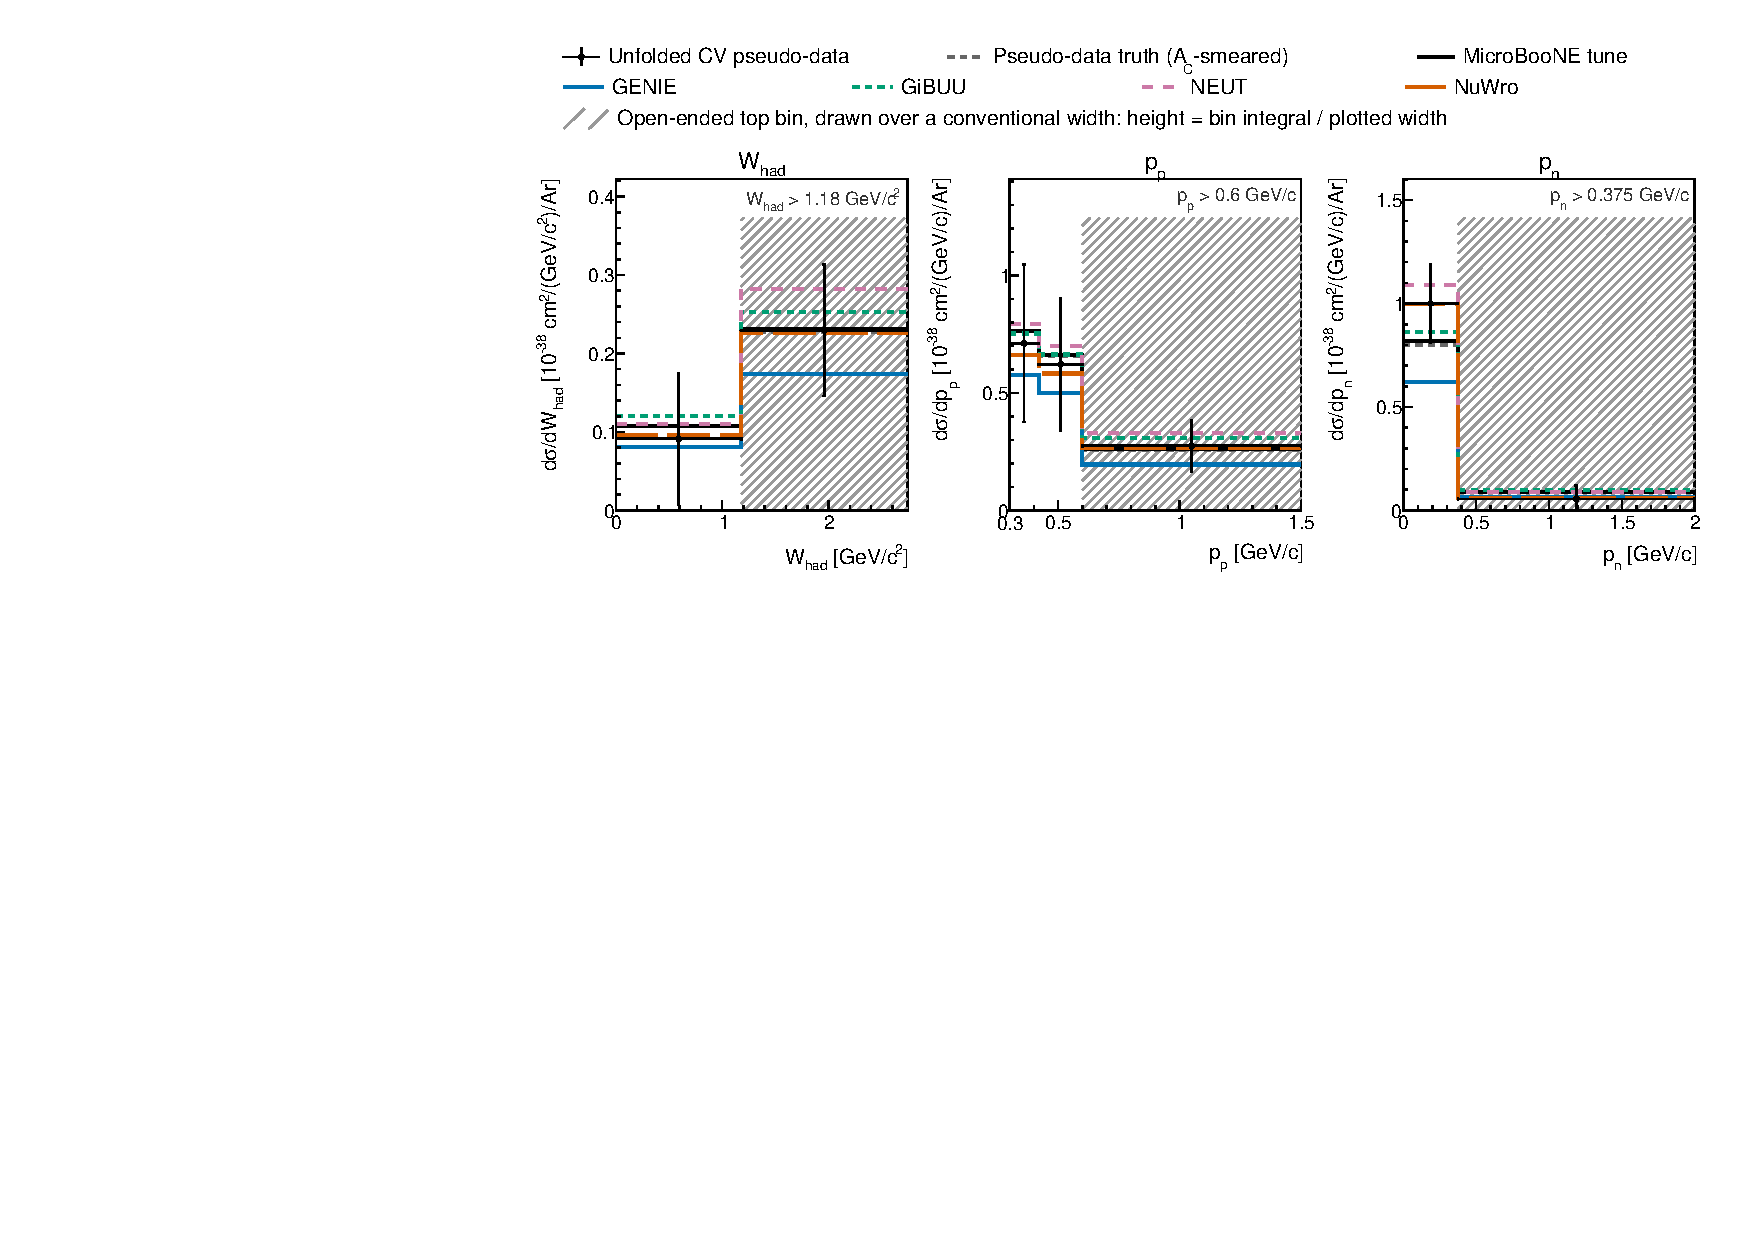
\includegraphics[width=\textwidth]{dsigma_ccpi1p_noW_COMB_a}
  \column{.38\textwidth}
  \begin{itemize}\footnotesize\setlength\itemsep{3pt}
    \item Combined configuration on pseudo-data: $W_{\rm had}$ 2 bins (split $1.18$~GeV), TKI 2--3 bins
          ($\delta p_T$ 2, $\delta\alpha_T$ split at $120^\circ$, $\delta\phi_T$ 3, $p_n$ 2), $p_p$ 3, $\theta_p$ 4,
          $\theta_{\pi p}$ 4.
    \item $W_{\rm had}$, TKI and $p_p$ are validation-only; the proton-tagged total, $\theta_p$, $\theta_{\pi p}$ and the
          $\theta_p\times\delta p_T$ 2D result are secondary.
    \item Open: inverted-proton-PID control region (P1), wrong-candidate term for $\theta_p$ (P2), model sensitivity of
          the low $\delta p_T$/$p_n$ bins (P3), $W_{\rm had}$/$p_n$ reconstruction validity (P4).
  \end{itemize}
  \end{columns}
\end{frame}

\begin{frame}{Documents and process}
  \begin{itemize}\small\setlength\itemsep{4pt}
    \item Three documents since 19 Sep: inclusive analysis note (approval path), proton-tagged note
          (validation), shared technical supplement; cross-referenced, one preamble.
    \item Review responses (27 Sep): status vocabulary, official covariance with the MCS term,
          \texttt{check\_documents.py} for consistency; approval material only in \texttt{approval\_request.tex}.
    \item Release packages with notes in \texttt{report/releases/release\_v1.*}; v1.6 for the Editorial Board
          (29 Sep), v1.6.1 errata (1 Oct), v1.7--v1.9 tagged 14 Oct.
    \item The documents of v1.6 to v1.9 describe the analysis before the control regions; 18 beam-on passages are held
          out until the control-region comparison is approved.
    \item PRD/PRL paper drafts started on 19 Sep, on hold since 15 Oct.
  \end{itemize}
\end{frame}

\begin{frame}{Open items}
  \begin{columns}[T]
  \column{.50\textwidth}
  \textbf{\color{ubred}Before unblinding}
  \begin{itemize}\footnotesize\setlength\itemsep{2pt}
    \item U1: written confirmation from the NuMI flux group that the flux constants are the PPFX-corrected central value.
    \item U2: control-region comparison under the frozen procedure approved; convener ratification of the procedure
          and the $\pi^0$ target; second-person skim verification.
    \item U3: independent-generator closure with a validated NuWro overlay.
    \item U5: beam-on POT and triggers per file checked against the beam database to $<1\%$.
    \item U6: clean-cache reproduction of the release to $10^{-9}$.
    \item FHC Run-1 residual: $13\pm2\%$ ($f=0.869\pm0.021$), cause not identified.
  \end{itemize}
  \column{.48\textwidth}
  \textbf{\color{ubred}Decisions and later}
  \begin{itemize}\footnotesize\setlength\itemsep{2pt}
    \item R1: collaboration decision on the combined-only 2D results.
    \item Adoption of the control-region conditional constraint ($35.8\%\to11.3\%$ on the total, Asimov).
    \item U7 (before publication): beamline-geometry flux term, beam-off gate-ratio term and the Run-2 beam-off
          stand-in term in the covariance.
    \item Proton-tagged P1--P4.
    \item Ensemble offset: the six inclusive 1D means are below the reference ($\leq0.9\%$, $\leq1.5\sigma$); the 2D
          $\cos\theta_\pi\times\cos\theta_\mu$ is $0.8\%$ low at $2.4\sigma$.
    \item U4 (MCS) complete with v1.9.
  \end{itemize}
  \end{columns}
\end{frame}

\begin{frame}{Summary}
  \begin{itemize}\small\setlength\itemsep{4pt}
    \item Four releases since the meeting. The central values on pseudo-data moved by less than $1\%$; the total
          uncertainty fell from about $38\%$ to $34$--$36\%$ (inclusive) through the fractional detector variations.
    \item Exposure and selection corrected where the beam-on control regions pointed: the FHC Run-1 exposure
          ($+14\%$ on $\sigma_{\rm FHC}$ for data), the Bragg-pion cut missing in the older productions ($4.7\%$ bias at
          unblinding avoided), the dirt in the count macros.
    \item Binnings now follow one criterion ($0.50$) for every released observable; new $\theta_p$, $\theta_{\pi p}$ and
          two 2D results, with status labels.
    \item The MCS momentum of exiting muons is calibrated from the control regions: every control-region shape test
          passes, the hold-out test transfers within the quoted term.
    \item Control regions with beam-on data: global $7.69/8$ ($p=0.46$). Open before unblinding: the flux constants,
          the approval of the control-region procedure, an independent-generator closure, the Run-1 residual.
  \end{itemize}
  \label{mainend}
\end{frame}

% ===========================================================================
\backuptrue
\appendix
\section*{Backup}

{\setbeamertemplate{footline}{}
\begin{frame}[plain]
  \begin{center}\Huge\color{ubred} Backup\end{center}
\end{frame}}

\begin{frame}{Backup: control-region shape tests with the calibrated simulation}
  \scriptsize\setlength{\tabcolsep}{4pt}
  \begin{columns}[T]
  \column{.48\textwidth}
  \begin{tabular}{llcc}
    \toprule
    Mode & Distribution & v1.7 & calibrated \\
    \midrule
    FHC & CC$0\pi$ $p_\mu$ & $13.29/6$ & $0.84/6$ \\
    FHC & cosmic $p_\mu$ & $5.36/6$ & $2.14/6$ \\
    FHC & multi-$\pi$ $p_\mu$ & $7.55/6$ & $3.77/6$ \\
    FHC & $\pi^0$ $p_\mu$ & $29.56/6$ & $3.83/6$ \\
    RHC & CC$0\pi$ $p_\mu$ & $50.01/6$ & $3.10/6$ \\
    RHC & cosmic $p_\mu$ & $7.83/6$ & $3.58/6$ \\
    RHC & multi-$\pi$ $p_\mu$ & $9.69/6$ & $1.14/6$ \\
    RHC & $\pi^0$ $p_\mu$ & $66.23/6$ & $2.05/6$ \\
    \midrule
    sum & $p_\mu$ & $189.52/48$ & $20.45/48$ \\
    sum & other distributions & $42.52/66$ & $42.52/66$ \\
    \bottomrule
  \end{tabular}
  \column{.48\textwidth}
  \begin{itemize}\footnotesize\setlength\itemsep{3pt}
    \item Beam-on data, frozen protocol, from \texttt{report/results/cr\_protocol\_mcscal.md}.
    \item The global normalisation $\chi^2$ is unchanged ($7.69/8$): the calibration moves events between $p_\mu$ bins,
          not between regions.
    \item Pseudo-data with the calibrated simulation: $p_\mu$ sum $22.9/48$, the reference for the data.
  \end{itemize}
  \end{columns}
\end{frame}

\begin{frame}{Backup: beam-off per run period}
  \centering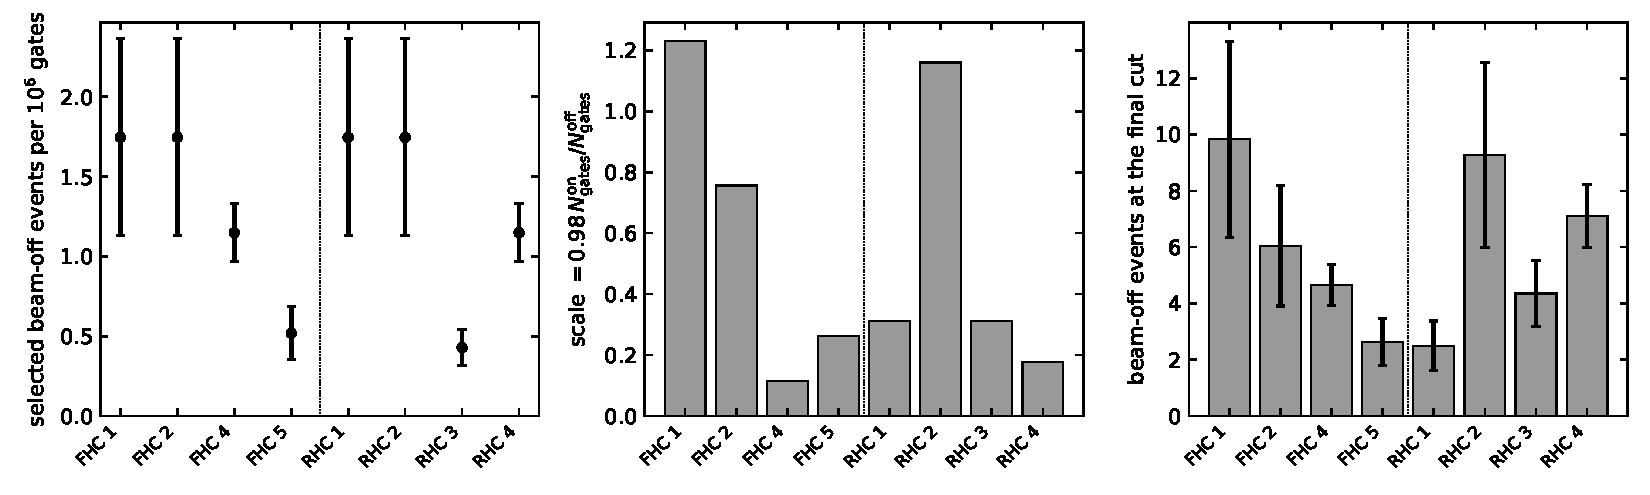
\includegraphics[width=0.92\textwidth]{ext_perrun_validation}\\[2mm]
  {\footnotesize Beam-off rate per run period with the corrected Run-1 trigger count.}
\end{frame}

\begin{frame}{Backup: two-dimensional results (combined)}
  \centering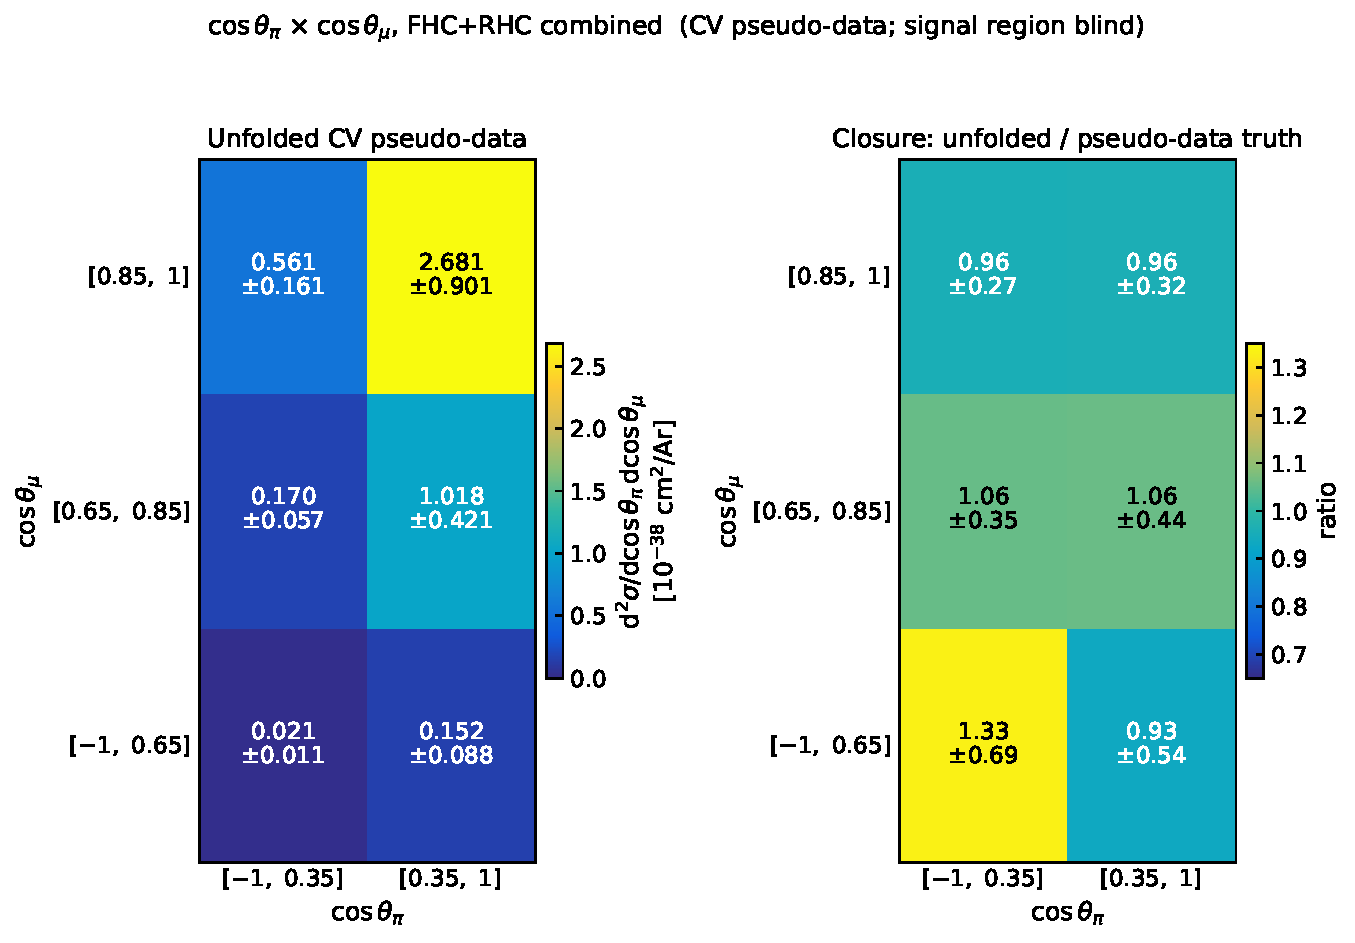
\includegraphics[width=0.48\textwidth]{bkgfit/xsec2d_costhpi_costhmu_COMB_map}\hfill
  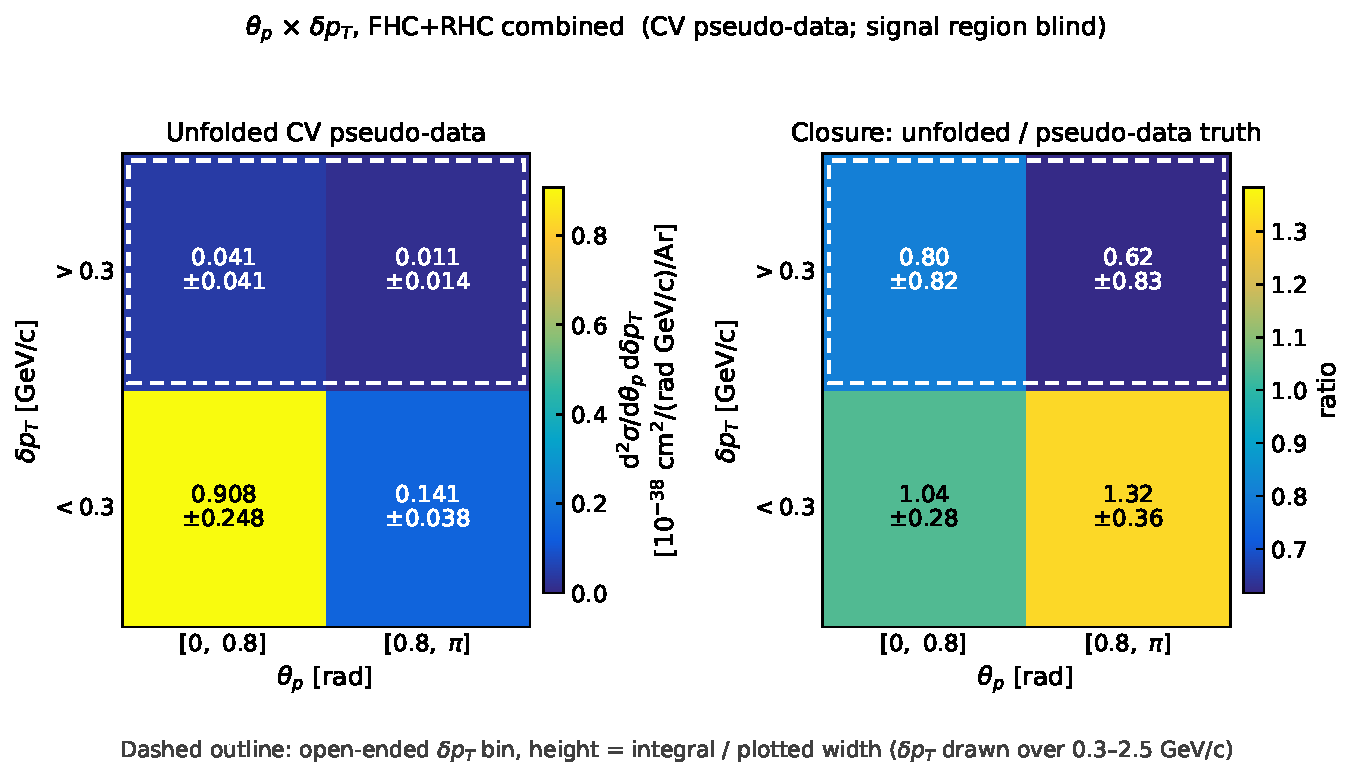
\includegraphics[width=0.48\textwidth]{bkgfit/xsec2d_thetap_dpt_COMB_map}\\[1mm]
  {\footnotesize $\cos\theta_\pi\times\cos\theta_\mu$ (6 cells, inclusive) and $\theta_p\times\delta p_T$ (4 cells,
  proton-tagged), unfolded pseudo-data and the tune; combined configuration only (R1).}
\end{frame}

\begin{frame}{Backup: uncertainty breakdown, FHC and RHC}
  \centering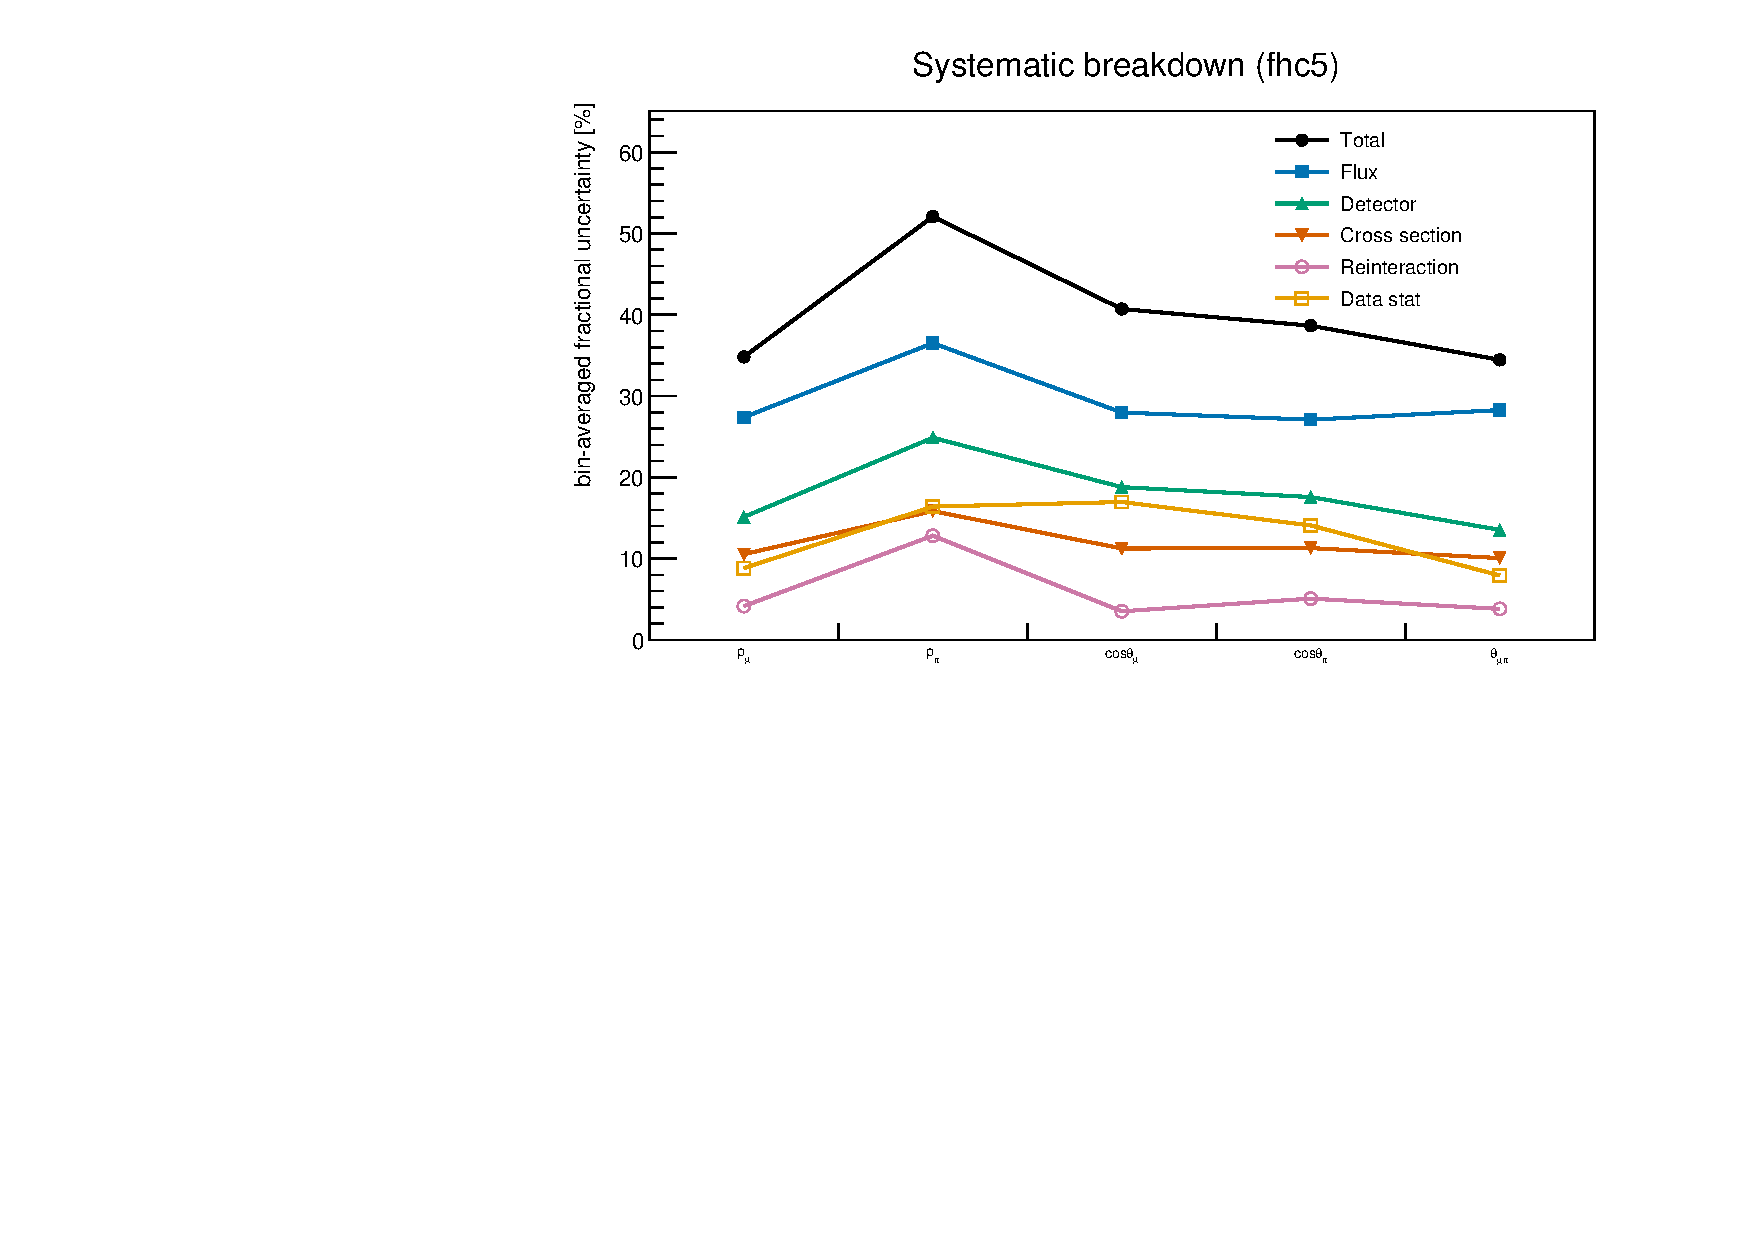
\includegraphics[width=0.48\textwidth]{fw_systbreak_fhc}\hfill
  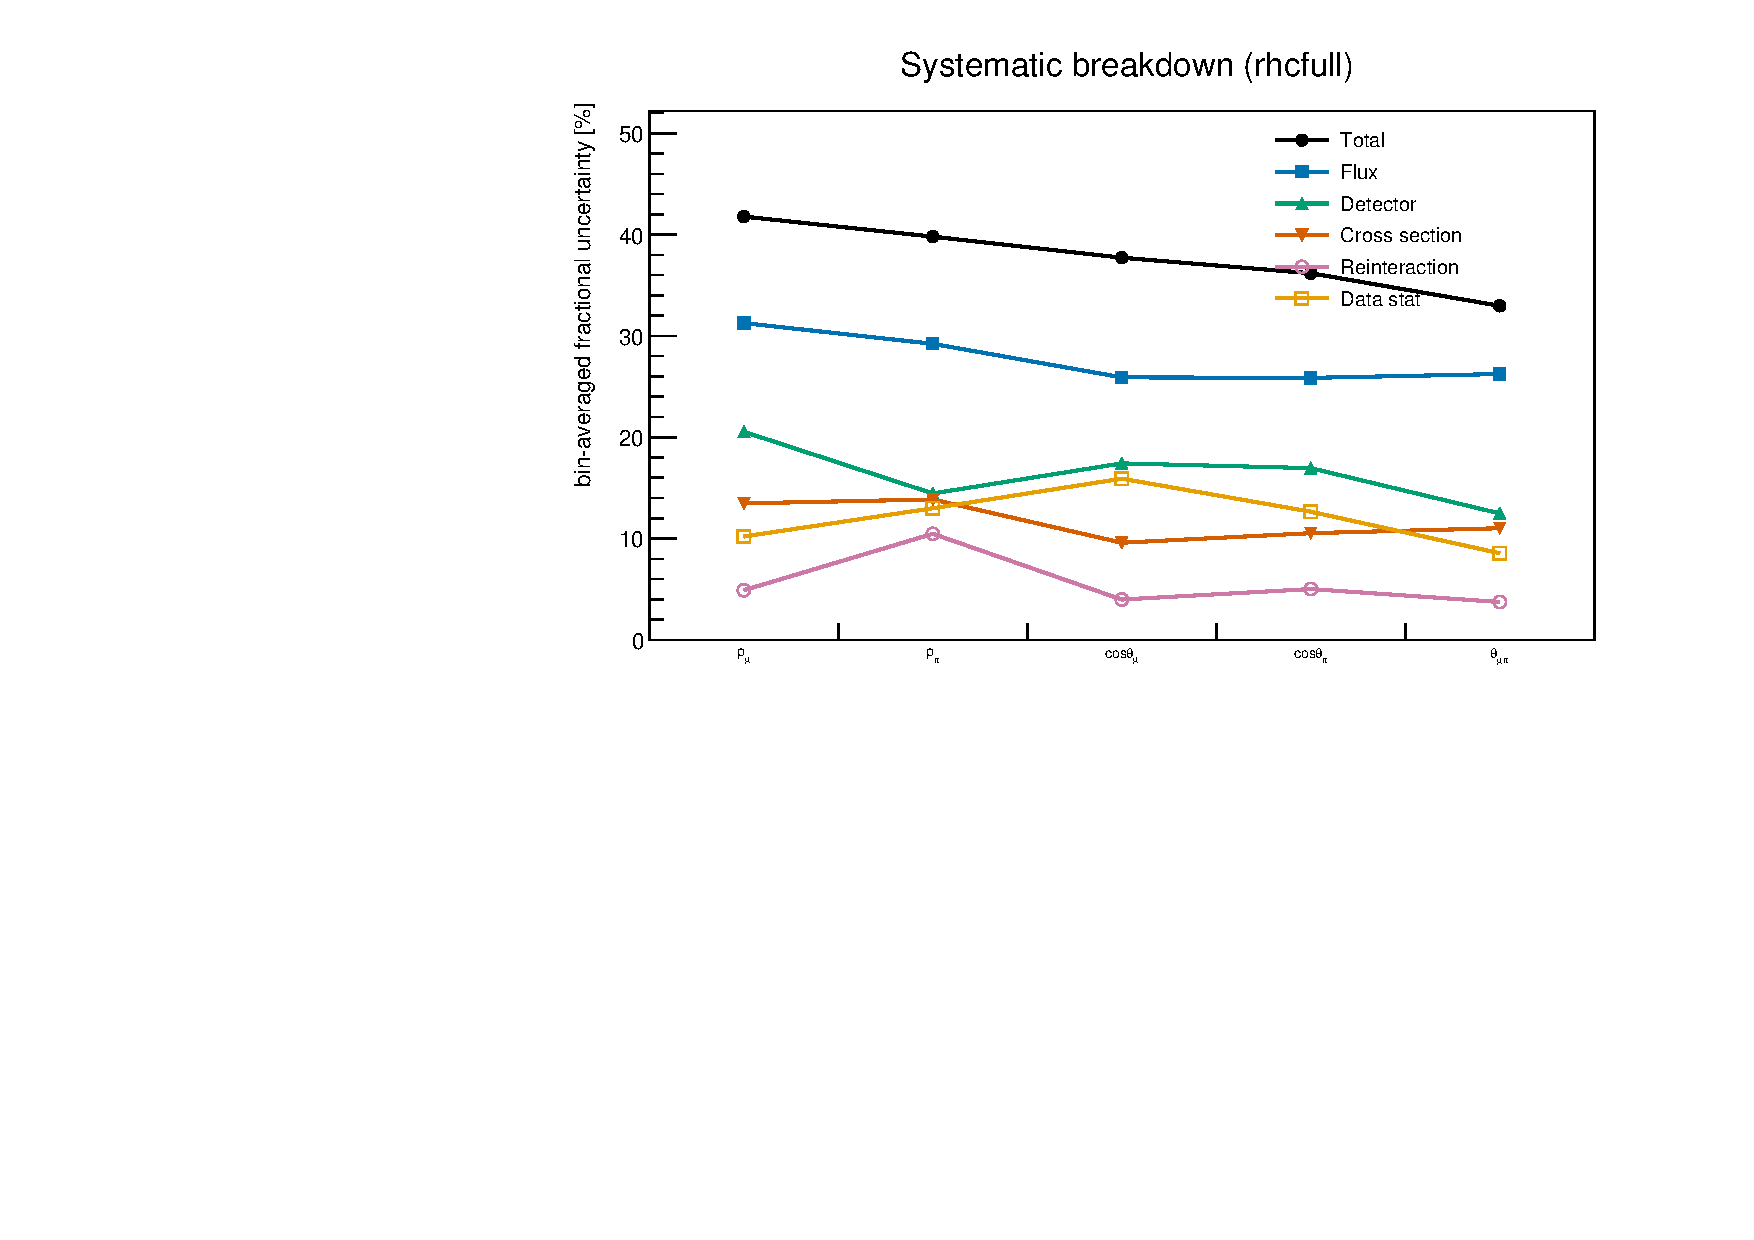
\includegraphics[width=0.48\textwidth]{fw_systbreak_rhc}
\end{frame}

\end{document}
